% chapters/07-local-network.tex

\chapter{Building Your Local Network}

\begin{importantbox}
This chapter provides strategies and frameworks for building effective local networks and partnerships in Nigeria, with specific guidance for different regions and sectors.
\end{importantbox}

\section{Partnership Strategy Framework}

\FloatBarrier
\subsection{Partner Types and Roles}
\begin{figure}[htbp]
    \centering
    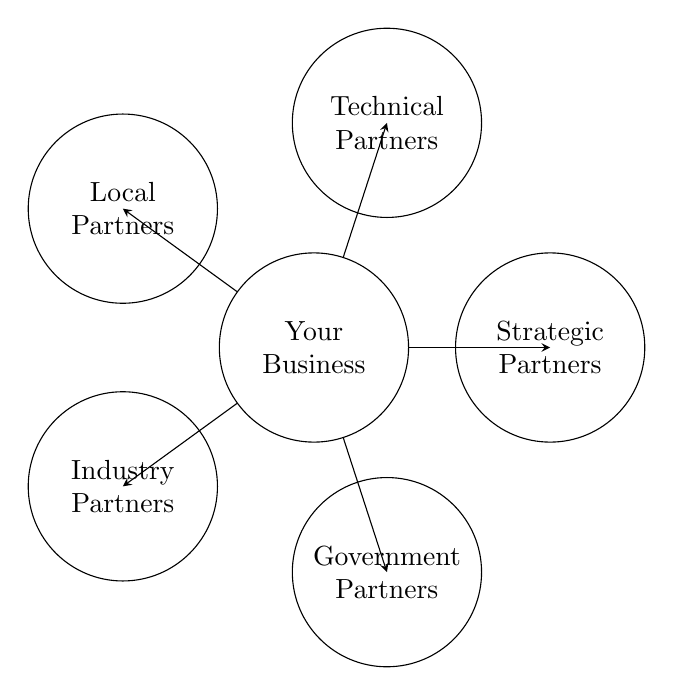
\begin{tikzpicture}[
        node distance=3cm,
        core/.style={draw, circle, text width=2cm, align=center},
        partner/.style={draw, circle, text width=2cm, align=center}
    ]
        % Partnership ecosystem diagram
        \node[core] (core) at (0,0) {Your\\Business};
        \foreach \angle/\label in {
            0/Strategic,
            72/Technical,
            144/Local,
            216/Industry,
            288/Government
        } {
            \node[partner] at (\angle:3) {\label\\Partners};
            \draw[-stealth] (core) -- (\angle:3);
        }
    \end{tikzpicture}
    \caption{Partnership Ecosystem}
    \label{fig:partnership-ecosystem}
\end{figure}

\subsection{Partnership Evaluation Matrix}
\begin{center}
\begin{tabularx}{\textwidth}{>{\raggedright\arraybackslash}X >{\centering\arraybackslash}X >{\centering\arraybackslash}X >{\raggedright\arraybackslash}X}
    \toprule
    \textbf{Partner Type} & \textbf{Value Add} & \textbf{Resource Need} & \textbf{Success Metrics} \\
    \midrule
    Strategic & Market access & High & Revenue growth \\
    Technical & Capabilities & Medium & Operation efficiency \\
    Local & Ground presence & Medium & Market penetration \\
    Industry & Credibility & Low & Sector recognition \\
    Government & Compliance & Medium & Regulatory ease \\
    \bottomrule
\end{tabularx}
\end{center}

\section{Key Stakeholder Mapping}

\subsection{Stakeholder Prioritization}
\begin{tcolorbox}[colback=white,colframe=primarydark,title=\textbf{Stakeholder Analysis}]
Priority Levels:
\begin{itemize}
    \item Critical: Immediate engagement required
    \item Important: Regular engagement needed
    \item Monitor: Periodic check-ins sufficient
    \item Inform: Keep updated on major developments
\end{itemize}
\end{tcolorbox}

\FloatBarrier
\section{Regional Network Development}

\begin{regionalbox}{United Kingdom}
\textbf{Financial and Property Networks}
\begin{itemize}
    \item Banking associations
    \item Investment groups
    \item Property developers
    \item Professional bodies
    \item UK-Nigeria chambers
\end{itemize}
\end{regionalbox}

\FloatBarrier
\subsection{UK Network Building Timeline}
\begin{figure}[htbp]
    \centering
    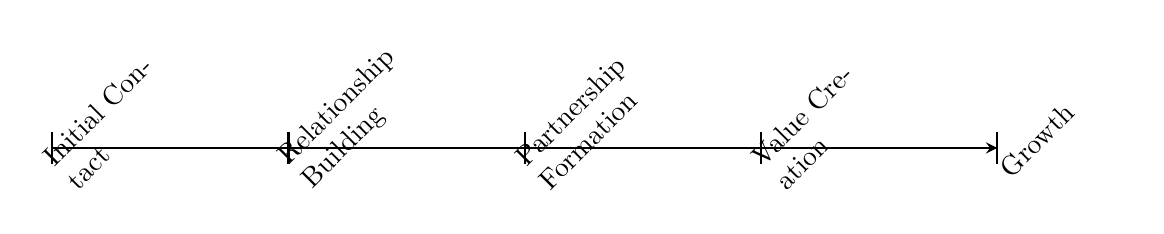
\begin{tikzpicture}[
        timeline/.style={thick, -stealth}
    ]
        % Network development timeline
        \draw[timeline] (0,0) -- (12,0);
        \foreach \x/\label in {
            0/Initial Contact,
            3/Relationship Building,
            6/Partnership Formation,
            9/Value Creation,
            12/Growth
        } {
            \draw[thick] (\x,0.2) -- (\x,-0.2);
            \node[text width=2cm, align=left, rotate=45, anchor=west]
                at (\x,-0.4) {\label};
        }
    \end{tikzpicture}
    \caption{UK Network Development Process}
    \label{fig:uk-network-timeline}
\end{figure}

\begin{regionalbox}{United States}
\textbf{Tech and Innovation Networks}
\begin{itemize}
    \item Tech hubs
    \item Startup communities
    \item Innovation centers
    \item Industry associations
    \item Venture networks
\end{itemize}
\end{regionalbox}

\FloatBarrier
\subsection{US Tech Ecosystem Map}
\begin{figure}[htbp]
    \centering
    \begin{tikzpicture}[
        node distance=2.5cm,
        box/.style={draw, minimum width=2.5cm, minimum height=1cm, align=center}
    ]
        % Tech ecosystem visualization with better spacing
        \node[box] (hub) at (0,0) {Tech Hub};
        \node[box] (accelerator) at (-3,-2.5) {Accelerators};
        \node[box] (investors) at (3,-2.5) {Investors};
        \node[box] (partners) at (0,-5) {Partners};

        % Add arrows with proper spacing
        \draw[-stealth] (hub) -- (accelerator);
        \draw[-stealth] (hub) -- (investors);
        \draw[-stealth] (accelerator) -- (partners);
        \draw[-stealth] (investors) -- (partners);
    \end{tikzpicture}
    \caption{US Tech Network Structure}
    \label{fig:us-tech-ecosystem}
\end{figure}

\begin{regionalbox}{UAE}
\textbf{Trade and Business Networks}
\begin{itemize}
    \item Trade associations
    \item Business councils
    \item Chamber of commerce
    \item Logistics networks
    \item Import/export groups
\end{itemize}

\subsection{UAE Trade Network Development}
\begin{tcolorbox}[colback=white,colframe=primary,title=\textbf{Network Building Steps}]
\begin{enumerate}
    \item Chamber membership
    \item Trade association participation
    \item Business council engagement
    \item Partner identification
    \item Relationship development
\end{enumerate}
\end{tcolorbox}
\end{regionalbox}

\begin{regionalbox}{Canada}
\textbf{Industry-Specific Communities}
\begin{itemize}
    \item Agricultural associations
    \item Environmental groups
    \item Technology clusters
    \item Research institutions
    \item Government agencies
\end{itemize}

\subsection{Canadian Sector Network Map}
\begin{center}
\begin{tabularx}{\textwidth}{>{\raggedright\arraybackslash}X >{\raggedright\arraybackslash}X >{\raggedright\arraybackslash}X}
    \toprule
    \textbf{Sector} & \textbf{Key Networks} & \textbf{Entry Points} \\
    \midrule
    Agriculture & Industry associations & Annual conferences \\
    Technology & Innovation hubs & Tech meetups \\
    Environment & Research groups & Sustainability forums \\
    \bottomrule
\end{tabularx}
\end{center}
\end{regionalbox}

\FloatBarrier
\section{Network Value Creation}

\subsection{Value Exchange Framework}
\begin{figure}[htbp]
    \centering
    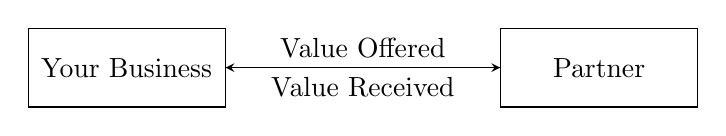
\begin{tikzpicture}[
        node distance=5cm,
        box/.style={draw, minimum width=2.5cm, minimum height=1cm, align=center}
    ]
        % Value exchange diagram with better spacing
        \node[box] (you) at (0,0) {Your Business};
        \node[box] (partner) at (6,0) {Partner};

        % Add arrows with labels
        \draw[-stealth] (you) -- node[above, text width=3cm, align=center] {Value Offered} (partner);
        \draw[-stealth] (partner) -- node[below, text width=3cm, align=center] {Value Received} (you);
    \end{tikzpicture}
    \caption{Partnership Value Exchange}
    \label{fig:value-exchange}
\end{figure}

\begin{communitybox}
Connect with partners and build your network on the Africa Growth Circle:
\begin{itemize}
    \item Partner directory
    \item Industry forums
    \item Networking events
    \item Expert introductions
    \item Partnership opportunities
\end{itemize}
Visit circle.counseal.com for networking support.
\end{communitybox}

% End of chapter workshop
\begin{workshopbox}
\textbf{Chapter 7 Network Building Workshop}

1. Network Mapping
\begin{itemize}
    \item Key stakeholders: \_\_\_\_\_\_\_\_\_
    \item Priority partners: \_\_\_\_\_\_\_\_\_
    \item Network gaps: \_\_\_\_\_\_\_\_\_
\end{itemize}

2. Partnership Planning
\begin{itemize}
    \item Target partners: \_\_\_\_\_\_\_\_\_
    \item Value proposition: \_\_\_\_\_\_\_\_\_
    \item Engagement strategy: \_\_\_\_\_\_\_\_\_
\end{itemize}

3. Relationship Development
\begin{itemize}
    \item Networking events: \_\_\_\_\_\_\_\_\_
    \item Introduction plans: \_\_\_\_\_\_\_\_\_
    \item Follow-up strategy: \_\_\_\_\_\_\_\_\_
\end{itemize}

Access the partner directory and networking tools on the Africa Growth Circle platform.
\end{workshopbox}

\begin{importantbox}
In Chapter 8, we'll explore the technology and operations setup needed to support your network and partnerships effectively.
\end{importantbox}